\documentclass[12pt]{article}

\usepackage{amsmath, mathtools}
\usepackage{amsfonts}
\usepackage{amssymb}
\usepackage{booktabs}
\usepackage{tabularx}
\usepackage{xspace}

\usepackage{graphicx}
\usepackage{colortbl}
\usepackage{xr}
\usepackage{longtable}
\usepackage{xfrac}
\usepackage{float}
\usepackage{siunitx}
\usepackage{caption}
\usepackage{pdflscape}
\usepackage{afterpage}

\usepackage{fullpage}
\usepackage[round]{natbib}
%\usepackage{refcheck}
\usepackage{lipsum}

%% Comments

\usepackage{color}

\newif\ifcomments\commentsfalse

\ifcomments
\newcommand{\authornote}[3]{\textcolor{#1}{[#3 ---#2]}}
\newcommand{\todo}[1]{\textcolor{red}{[TODO: #1]}}
\else
\newcommand{\authornote}[3]{}
\newcommand{\todo}[1]{}
\fi

\newcommand{\wss}[1]{\authornote{blue}{SS}{#1}} 
\newcommand{\plt}[1]{\authornote{magenta}{TPLT}{#1}} %For explanation of the template
\newcommand{\an}[1]{\authornote{cyan}{Author}{#1}}
\newcommand{\jme}[1]{\authornote{cyan}{JME}{#1}}

% Common Parts

\usepackage{tabularx}
\usepackage{booktabs}
\usepackage{ifthen}
\usepackage{amsmath,amssymb,xspace}

%PUT YOUR PROGRAM NAME HERE %Every program should have a name
\newcommand{\progname}[1]
{%
  \ifthenelse{\equal{#1}{n}}{{\normalsize ROC\xspace}}{}%
  \ifthenelse{\equal{#1}{L}}{{\Large ROC\xspace}}{}%
  \ifthenelse{\equal{#1}{f}}{{\footnotesize ROC\xspace}}{}%
}
% Abbreviations
\newcommand{\ode}{{\footnotesize ODE}\xspace}
\newcommand{\dae}{{\footnotesize DAE}\xspace}
\newcommand{\ivp}{{\footnotesize IVP}\xspace}
\newcommand{\fadbad}{{\footnotesize FADBAD++}\xspace}
\newcommand{\plainc}{{\footnotesize C}\xspace}
\newcommand{\cpp}{{\footnotesize C++}\xspace}
\newcommand{\adolc}{{\footnotesize ADOL-C}\xspace}
\newcommand{\rdcon}{{\footnotesize DRDCV}\xspace}
\newcommand{\fortran}{{\footnotesize FORTRAN 77}\xspace}
\newcommand{\daets}{{\footnotesize DAETS}\xspace}
\newcommand{\matlab}{{\footnotesize MATLAB}\xspace}
\newcommand{\mathematica}{{\footnotesize MATHEMATICA}\xspace}
\newcommand{\maple}{{\footnotesize MAPLE}\xspace}
% User commands
\newcommand{\Quote}[1]{``{#1}''}
\newcommand{\Ni}{\noindent}
% Environment
\newcommand{\EQ}[1]{\begin{align} {#1} \end{align}}
% Mathematics
\newcommand{\parn}[1]{( {#1} )}
\newcommand{\parbg}[1]{\left(  {#1} \right)}
\newcommand{\pbg}[1]{\bigl(  {#1} \bigr)}
\newcommand{\Setbg}[1]{\bigl\{ {#1} \bigr\}}
\def\Rz{\mathbb{R}}
\def\Cz{\mathbb{C}}
\newcommand{\nliminf}[1]{\liminf\limits_{{#1} \rightarrow \infty}}
\newcommand{\nlimsup}[1]{\limsup\limits_{{#1} \rightarrow \infty}}
% Mathematics: ODE
\newcommand{\iode}{\protect{\makebox{$[t_0,\tend]$}}\xspace}
\newcommand{\lode}{\protect{\makebox{$[t_n,t_{n+1}]$}}\xspace}
\newcommand{\tend}{t_\text{end}}
\newcommand{\tc}[2]{(#1)_{#2}}
\newcommand{\Tp}{T}
\newcommand{\xn}{x_{n}}
\newcommand{\tn}{t_{n}}
% Reference
\renewcommand{\eqref}[1]{(\ref{eq:#1})}
\newcommand{\rrf}[2]{(\ref{eq:#1}--\ref{eq:#2})}
\newcommand{\chref}[1]{\ref{ch:#1}}
\newcommand{\sscref}[1]{\ref{ssc:#1}}
\newcommand{\scref}[1]{Section~\ref{sc:#1}}
\newcommand{\exref}[1]{\ref{ex:#1}}
\newcommand{\rmref}[1]{\ref{rm:#1}}
\newcommand{\apref}[1]{\ref{ap:#1}}
%\newcommand{\tbref}[1]{\ref{tb:#1}}
\newcommand{\dfref}[1]{\ref{df:#1}}
\newcommand{\leref}[1]{\ref{le:#1}}
\newcommand{\fgref}[1]{\ref{fg:#1}}
\newcommand{\coref}[1]{\ref{co:#1}}
\newcommand{\thref}[1]{\ref{th:#1}}
\newcommand{\agref}[1]{\ref{ag:#1}}
\newcommand{\asref}[1]{\ref{as:#1}}
\newcommand{\EQref}[1]{Equation~(\ref{eq:#1})}
\newcommand{\CHref}[1]{Chapter~\ref{ch:#1}}
\newcommand{\SSCref}[1]{Subsection~\ref{ssc:#1}}
\newcommand{\SCref}[1]{Section~\ref{sc:#1}}
\newcommand{\EXref}[1]{Example~\ref{ex:#1}}
\newcommand{\RMref}[1]{Remark~\ref{rm:#1}}
\newcommand{\APref}[1]{Appendix~\ref{ap:#1}}
\newcommand{\TBref}[1]{Table~\ref{tb:#1}}
\newcommand{\DFref}[1]{Definition~\ref{df:#1}}
\newcommand{\LEref}[1]{Lemma~\ref{le:#1}}
\newcommand{\FGref}[1]{Figure~\ref{fg:#1}}
\newcommand{\COref}[1]{Corollary~\ref{co:#1}}
\newcommand{\THref}[1]{Theorem~\ref{th:#1}}
\newcommand{\AGref}[1]{Algorithm~\ref{ag:#1}}
\newcommand{\ASref}[1]{Assumption~\ref{as:#1}}



% For easy change of table widths
\newcommand{\colZwidth}{1.0\textwidth}
\newcommand{\colAwidth}{0.13\textwidth}
\newcommand{\colBwidth}{0.82\textwidth}
\newcommand{\colCwidth}{0.1\textwidth}
\newcommand{\colDwidth}{0.05\textwidth}
\newcommand{\colEwidth}{0.8\textwidth}
\newcommand{\colFwidth}{0.17\textwidth}
\newcommand{\colGwidth}{0.5\textwidth}
\newcommand{\colHwidth}{0.28\textwidth}

% Used so that cross-references have a meaningful prefix
\newcounter{defnum} %Definition Number
\newcommand{\dthedefnum}{GD\thedefnum}
\newcommand{\dref}[1]{GD\ref{#1}}
\newcounter{datadefnum} %Datadefinition Number
\newcommand{\ddthedatadefnum}{DD\thedatadefnum}
\newcommand{\ddref}[1]{DD\ref{#1}}
\newcounter{theorynum} %Theory Number
\newcommand{\tthetheorynum}{T\thetheorynum}
\newcommand{\tref}[1]{TM\ref{#1}}
\newcounter{tablenum} %Table Number
\newcommand{\tbthetablenum}{T\thetablenum}
\newcommand{\tbref}[1]{TB\ref{#1}}
\newcounter{assumpnum} %Assumption Number
\newcommand{\atheassumpnum}{P\theassumpnum}
\newcommand{\aref}[1]{A\ref{#1}}
\newcounter{goalnum} %Goal Number
\newcommand{\gthegoalnum}{P\thegoalnum}
\newcommand{\gsref}[1]{GS\ref{#1}}
\newcounter{instnum} %Instance Number
\newcommand{\itheinstnum}{IM\theinstnum}
\newcommand{\iref}[1]{IM\ref{#1}}

\newcounter{reqnum} %Requirement Number
\newcommand{\rthereqnum}{R\thereqnum}
\newcommand{\rref}[1]{R\ref{#1}}
\newcommand{\rlabel}[1]{\refstepcounter{reqnum} \rthereqnum \label{#1}:}

\newcounter{lcnum} %Likely change number
\newcommand{\lthelcnum}{LC\thelcnum}
\newcommand{\lcref}[1]{LC\ref{#1}}

\begin{document}

\title{Software Requirements Specification for \progname{L}: Software estimating the radius of convergence of
a power series} 
\author{John M Ernsthausen}
\date{\today}
	
\maketitle

~\newpage

\pagenumbering{roman}

\tableofcontents

~\newpage

\section*{Revision History}

\begin{tabularx}{\textwidth}{p{3cm}p{2cm}X}
\toprule {\bf Date} & {\bf Version} & {\bf Notes}\\
\midrule
12 October 2020 & 1.0 & First submission\\
\bottomrule
\end{tabularx}

~\newpage

\section{Reference Material}

This section records information for easy reference.

\subsection{Table of Units}

A Table of Units is not applicable to \progname{f}.

\plt{
Throughout this document SI (Syst\`{e}me International d'Unit\'{e}s) is employed
as the unit system.  In addition to the basic units, several derived units are
used as described below.  For each unit, the symbol is given followed by a
description of the unit and the SI name.
~\newline

\renewcommand{\arraystretch}{1.2}
%\begin{table}[ht]
  \noindent \begin{tabular}{l l l} 
    \toprule		
    \textbf{symbol} & \textbf{unit} & \textbf{SI}\\
    \midrule 
    \si{\metre} & length & metre\\
    \si{\kilogram} & mass	& kilogram\\
    \si{\second} & time & second\\
    \si{\celsius} & temperature & centigrade\\
    \si{\joule} & energy & joule\\
    \si{\watt} & power & watt (W = \si{\joule\per\second})\\
    \bottomrule
  \end{tabular}
  %	\caption{Provide a caption}
%\end{table}
}

\plt{Only include the units that your SRS actually uses.}

\plt{Derived units, like newtons, pascal, etc, should show their derivation
    (the units they are derived from) if their constituent units are in the
    table of units (that is, if the units they are derived from are used in the
    document).  For instance, the derivation of pascals as
    $\si{\pascal}=\si{\newton\per\square\meter}$ is shown if newtons and m are
    both in the table.  The derivations of newtons would not be shown if kg and
    s are not both in the table.}

\plt{The symbol for units named after people use capital letters, but the name
  of the unit itself uses lower case.  For instance, pascals use the symbol Pa,
  watts use the symbol W, teslas use the symbol T, newtons use the symbol N,
  etc.  The one exception to this is degree Celsius.  Details on writing metric
  units can be found on the 
  \href{https://www.nist.gov/pml/weights-and-measures/writing-metric-units}
  {NIST} web-page.}

\subsection{Table of Symbols}

The table that follows summarizes the mathematical notation used in this document.
%The symbols are listed in alphabetical order.


\renewcommand{\arraystretch}{1.2}
%\noindent \begin{tabularx}{1.0\textwidth}{l l X}
\noindent \begin{longtable*}{l p{12cm}} \toprule
\textbf{symbol} & \textbf{description}\\
\midrule
  $z \in \Cz$ & A member $z$ of the complex numbers $\Cz$\\
  $x \in \Rz$ & A member $x$ of the real numbers $\Rz$\\
  $\Setbg{c_n} \subset \Cz$ & A sequence of complex numbers
  whose $n^\text{th}$ term is $c_n \in \Cz$\\
  $\Setbg{c_n}_{n=0}^{N-1} \subset \Cz$ & A finite sequence of $N$ complex numbers
  whose $n^\text{th}$ term is $c_n \in \Cz$\\
  $\sum_{n=0}^{\infty} c_n (z-z_0)^n$ & A power series. $c_n \in \Cz$ is the
  $n^\text{th}$ coefficient. $z^n$ is the $n^\text{th}$ power of $z \in \Cz$. $z_0$ is the center point.\\ 
  $\nliminf{n}$ & Lower subsequential limit\\
  $\nlimsup{n}$ & Upper subsequential limit\\
  $R_c$ & Radius of the circle of convergence\\
  $\Rz^d$ & A $d$-dimension real vector space\\
  $\mathcal D$ & An open subset of $\Rz^d$\\
  $[a,b] \subset \Rz$ & Interval of real numbers, $t \in [a,b]$ means $a \leq t \leq b$ and $t \in \Rz$\\
  $\tc{\xn}{n}$ & $n^\text{th}$ Taylor coefficient of $t \in \Rz \mapsto x \in \Rz^d$ evaluated at $t_n \in \Rz$\\
\bottomrule
\end{longtable*}

\plt{Use your problems actual symbols.  The si package is a good idea to use for
  units.}

\subsection{Abbreviations and Acronyms}

\renewcommand{\arraystretch}{1.2}
\begin{tabular}{l l} 
  \toprule		
  \textbf{symbol} & \textbf{description}\\
  \midrule 
  A & Assumption\\
  $\Cz$ & Complex numbers\\
  DD & Data Definition\\
  GD & General Definition\\
  GS & Goal Statement\\
  IM & Instance Model\\
  \ivp & Initial Value Problem\\
  LC & Likely Change\\
  $\Iz$ & The non-negative integers\\
  \ode & Ordinary Differential Equation\\
  $\Rz$ & Real numbers\\
  R & Requirement\\
  \progname{f} & Radius of Convergence software developed for this project\\
  SRS & Software Requirements Specification\\
  T & Theoretical Model\\
  TC & Taylor coefficient\\
  TS & Taylor series\\
  \bottomrule
\end{tabular}\\

% \plt{Add any other abbreviations or acronyms that you add}

\newpage

\pagenumbering{arabic}

\plt{This SRS template is based on \citet{SmithAndLai2005, SmithEtAl2007}.  It
  will get you started.  You should not modify the section headings, without
  first discussing the change with the course instructor.  Modification means
  you are not following the template, which loses some of the advantage of a
  template, especially standardization.  Although the bits shown below do not
  include type information, you may need to add this information for your
  problem.  If you are unsure, please can ask the instructor.}

\plt{Feel free to change the appearance of the report by modifying the LaTeX
  commands.}

\plt{This template document assumes that a single program is being documented.
  If you are documenting a family of models, you should start with a commonality
  analysis.  A separate template is provided for this.  For program
  families you should look at \cite{Smith2006, SmithMcCutchanAndCarette2017}.
  Single family member programs are often programs based on a single physical
  model.  General purpose tools are usually documented as a family.  Families of
  physical models also come up.}

\plt{The SRS is not generally written, or read, sequentially.  The SRS is a
  reference document.  It is generally read in an ad hoc order, as the need
  arises.  For writing an SRS, and for reading one for the first time, the
  suggested order of sections is:
\begin{itemize}
\item Goal Statement
\item Instance Models
\item Requirements
\item Introduction
\item Specific System Description
\end{itemize}
}

\plt{Guiding principles for the SRS document:
\begin{itemize}
\item Do not repeat the same information at the same abstraction level.  If
  information is repeated, the repetition should be at a different abstraction
  level.  For instance, there will be overlap between the scope section and the
  assumptions, but the scope section will not go into as much detail as the
  assumptions section.
\end{itemize}
}

\plt{The template description comments should be disabled before submitting this
  document for grading.}

\plt{You can borrow any wording from the text given in the template.  It is part
  of the template, and not considered an instance of academic integrity.  Of
  course, you need to cite the source of the template.}

\plt{When the documentation is done, it should be possible to trace back to the
  source of every piece of information.  Some information will come from
  external sources, like terminology.  Other information will be derived, like
  General Definitions.}

\plt{An SRS document should have the following qualities: unambiguous,
  consistent, complete, validatable, abstract and traceable.}

\plt{The overall goal of the SRS is that someone that meets the Characteristics
  of the Intended Reader (Section~\ref{sec_IntendedReader}) can learn,
  understand and verify the captured domain knowledge.  They should not have to
  trust the authors of the SRS on any statements.  They should be able to
  independently verify/derive every statement made.}

%CHAPTER
\section{Introduction} \label{sc:introduction}

Given a sequence $\Setbg{c_n}$ of complex numbers, the series
\EQ
{
  \label{eq:power-series}
  \sum_{n=0}^{\infty} c_n (z-z_0)^n
}
is called a {\it power series}. The number $c_n  \in \Cz$ is the $n^\text{th}$ coefficient in the power series.
The symbol $z^n$ denotes the $n^\text{th}$ power of the complex number $z$. This power series is {\it centered}
at $z_0 \in \Cz$.

In general, a power series will converge or diverge, depending on the magnitude of $z-z_0$.
With every power series, there is associated a circle of convergence such that
\eqref{power-series} converges if $z$ is in the interior of the circle of convergence or
diverges if $z$ is in the exterior of the circle of convergence. The convergence/divergence
behavior of \eqref{power-series} on the circle of convergence can not be described so simply.
By convention, the entire complex plane is the interior of a circle of infinite radius, and a
point is the interior of a circle of zero radius.

This project is concerned with estimating the radius $R_c$ of the circle of convergence.

\plt{The introduction section is written to introduce the problem.  It starts
  general and focuses on the problem domain. The general advice is to start with
a paragraph or two that describes the problem, followed by a ``roadmap''
paragraph.  A roadmap orients the reader by telling them what sub-sections to
expect in the Introduction section.}

\subsection{Purpose of Document}

The purpose of this document is to facilitate communication between the stakeholders and developers
 during the software development of project \progname{f}
 %design, software development and testing, verification and validation, and documentation of \progname{f}
 by communicating and reflecting its software requirements.
The scientific and business problem \progname{f} solves is described in
Section~\ref{Sec_pd}, the \Quote{Problem~Description}. 

\plt{This section summarizes the purpose of the SRS document.  It does not focus
  on the problem itself.  The problem is described in the ``Problem
  Description'' section (Section~\ref{Sec_pd}).  The purpose is for the document
  in the context of the project itself, not in the context of the CAS 741
  course.  Although the ``purpose'' of the document is to get a grade in 741,
  you should not mention this.  Instead, ``fake it'' as if this is a real
  project.  The purpose section will be similar between projects.  The purpose
  of the document is the purpose of the SRS, including communication, planning
  for the design stage, etc.}

\subsection{Scope of Requirements}\label{sc:scope}

In the late 1800's, several authors resolved problems
concerning the characterization and analysis of singularities for power series.
\cite{chang1982} discuss this history, the topic of the following quote.

\begin{quote}
Our approach to series analysis was motivated by the observation that series
for solutions to \ode{s} follow a few very definite patterns which are characterized
by the location of primary singularities. In general, the coefficients of a power
series follow no patterns, so few theorems about truncated series can be proved.
However, series which are real-valued on the real axis can have poles, logarithmic
branch points, and essential singularities only on the real axis or in conjugate pairs.
Further, the effects of all secondary singularities disappear if sufficiently
  long series are used.  \citep[p.~122]{chang1982}
\end{quote}

A primary singularity of \eqref{power-series} is the closest singularity to the series
expansion point $z_0$ in the complex plane. All other singularities are secondary singularities.

\cite{chang1982} proposed a method of four parts to estimate the radius $R_c$ of the circle of convergence
as well as the order and location of primary singularities. The top-hump analysis applies to
the power series of entire functions. The 3-term analysis applies to the power series of
functions exhibiting a single primary singularity. The 6-term analysis applies to the
power series of functions exhibiting a conjugate pair of primary singularities.
Whenever these three analysis fail to resolve the $R_c$, singularity order, and
singularity location parameters for the series, the \cite{chang1982} method does
a top-line analysis. Each \cite{chang1982} sub-method works by fitting $R_c$, singularity order, and
singularity location parameters of a known model to the given sequence.

Top-line analysis always applies to power series. It resolves situations where secondary singularities are
less distinguishable from primary singularities. However it is less accurate, but it does
have a convergence analysis \citep{chang1982}.

The scope of this \progname{f} project is limited to top-line analysis.

\plt{Modelling the real world requires simplification.  The full complexity of
  the actual physics, chemistry, biology is too much for existing models, and
  for existing computational solution techniques.  Rather than say what is in
  the scope, it is usually easier to say what is not.  You can think of it as
  the scope is initially everything, and then it is constrained to create the
  actual scope.  For instance, the problem can be restricted to 2 dimensions, or
  it can ignore the effect of temperature (or pressure) on the material
  properties, etc.}  

\plt{The scope section is related to the assumptions section
  (Section~\ref{sec_assumpt}).  However, the scope and the assumptions are not
  at the same level of abstraction.  The scope is at a high level.  The focus is
  on the ``big picture'' assumptions.  The assumptions section lists, and
  describes, all of the assumptions.}

\subsection{Characteristics of Intended Reader} \label{sec_IntendedReader}

This document assumes the intended reader has familiarity with basic real analysis, complex analysis,
and Taylor arithmetic.
Courses which contribute to background knowledge may be titled Ordinary Differential Equations and
Linear Algebra (undergrad), Introduction to Real Analysis (undergrad),
Multivariate Calculus (undergrad), Functional Analysis (Graduate), Real Analysis (Graduate),
and Complex Analysis (Graduate).
Sequences and power series as well as the ratio and root tests will be discussed
in this document. However, our exposition will only cover the concepts needed for our purposes. For proofs
and for a complete exposition of all background materials, the interested reader should consult a beginning
level graduate text such as \cite{rudin1976}. For a brief but sufficient introduction to Taylor arithmetic,
consult \cite{TADIFF}.


\plt{This section summarizes the skills and knowledge of the readers of the
  SRS.  It does NOT have the same purpose as the ``User Characteristics''
  section (Section~\ref{SecUserCharacteristics}).  The intended readers are the
  people that will read, review and maintain the SRS.  They are the people that
  will conceivably design the software that is intended to meet the
  requirements.  The user, on the other hand, is the person that uses the
  software that is built.  They may never read this SRS document.  Of course,
  the same person could be a ``user'' and an ``intended reader.''}

\plt{The intended reader characteristics should be written as unambiguously and
  as specifically as possible.  Rather than say, the user should have an
  understanding of physics, say what kind of physics and at what level.  For
  instance, is high school physics adequate, or should the reader have had a
  graduate course on advanced quantum mechanics?}

\subsection{Organization of Document}

This document is built on the template recommendations in \citet{SmithAndLai2005, SmithEtAl2007} that
 seeks to standardize communication tools for software development. The suggested order for reading
 this SRS document is: Goal Statement (\SSCref{goal-statements}), Instance Models (\SSCref{instance-models}),
 Requirements (\SCref{requirements}), Introduction (\SCref{introduction}), and
 Specific System Description (\SCref{specific-system-description}).


\plt{This section provides a roadmap of the SRS document.  It will help the
  reader orient themselves.  It will provide direction that will help them
  select which sections they want to read, and in what order.  This section will
  be similar between project.}

%CHAPTER
\section{General System Description}

This section provides general information about the system.  It identifies the
interfaces between the system and its environment, describes the user
characteristics, and lists the system constraints.  \plt{This text can likely be
  borrowed verbatim.}

\plt{The purpose of this section is to provide general information about the
  system so the specific requirements in the next section will be easier to
  understand. The general system description section is designed to be
  changeable independent of changes to the functional requirements documented in
  the specific system description. The general system description provides a
  context for a family of related models.  The general description can stay the
  same, while specific details are changed between family members.}

\subsection{System Context}\label{ssc:systemcontext}

The following figure depicts a system context view of \progname{f}. This
context appears, for example, in the numerical solution of ordinary differential and
differential algebraic equations.

\begin{figure}[h!]
\begin{center}
 
\includegraphics[width=0.95\textwidth]{roc-system-context}
\caption{System Context}
\label{fg:systemcontext} 
\end{center}
\end{figure}

After generating a real-valued Taylor series (TS) approximate solution of order $p$ to the
ordinary differential equation (\ode) initial-value problem (\ivp) 
\EQ
{
  \label{eq:introduction-mathematical-odeivp}
  y'\parn{t} = f\pbg{t,y\parn{t}},
  \quad
  y\parn{t_0} = y_0 \in \mathcal D \subset \Rz^d,
  \quad
  t \in \iode \subset \Rz,
}
the TS methods defined in
\cite{jorba2005software},
\cite{bergsma2016application},
and \cite{chang1982} explicitly require an estimate for the TS radius of convergence.

% From a practical standpoint, an order $1 \leq p \leq k$ TS approximate solution requires
% $\parbg{t,y} \mapsto f\parbg{t,y} \in \Rz^d$ to be $k$-times differentiable.
% \cite{jorba2005software} permit the order $p$ to change from step to step.
At each $\parn{t_n,x_n}$, $n \geq 0$, the TS method for the numerical solution
of \eqref{introduction-mathematical-odeivp} computes Taylor coefficients (TCs)
$\tc{\xn}{i}$ at $t_{n}$ to construct the TS approximate solution
\begin{align}
  \label{eq:tss}
  \Tp(t) = \xn + \sum_{i=1}^{p}\tc{\xn}{i}(t-\tn)^{i} \quad\mbox{on}\quad \lode.
\end{align}
Analysis of \EQref{tss} for its radius of convergence provides a practical system
context for \progname{f} as depicted in \FGref{systemcontext}.
In this system context, developers like \cite{bergsma2016application},
\cite{jorba2005software}, or \cite{chang1982} of a TS method seek the accuracy
assurance from knowing the domain $\lode$ is in the circle of convergence.

\plt{Your system context will include a figure that shows the abstract view of
  the software.  Often in a scientific context, the program can be viewed
  abstractly following the design pattern of Inputs $\rightarrow$ Calculations
  $\rightarrow$ Outputs.  The system context will therefore often follow this
  pattern.  The user provides inputs, the system does the calculations, and then
  provides the outputs to the user.  The figure should not show all of the
  inputs, just an abstract view of the main categories of inputs (like material
  properties, geometry, etc.).  Likewise, the outputs should be presented from
  an abstract point of view.  In some cases the diagram will show other external
  entities, besides the user.  For instance, when the software product is a
  library, the user will be another software program, not an actual end user.}

\plt{
\begin{figure}[h!]
\begin{center}
 
\includegraphics[width=0.6\textwidth]{roc-system-context}
\caption{System Context}
\label{fig:systemcontext} 
\end{center}
\end{figure}
}

\plt{For each of the entities in the system context diagram its responsibilities
  should be listed.  Whenever possible the system should check for data quality,
  but for some cases the user will need to assume that responsibility.}

\plt{
\begin{itemize}
\item User Responsibilities:
\begin{itemize}
\item 
\end{itemize}
\item \progname{} Responsibilities:
\begin{itemize}
\item Detect data type mismatch, such as a string of characters instead of a
  floating point number
\item 
\end{itemize}
\end{itemize}
}

\subsection{User Characteristics} \label{SecUserCharacteristics}
\label{sc:SecUserCharacteristics}

One intended user of \progname{f} is a user of \maple or \matlab. While
neither \matlab nor \maple currently implements an estimate for $R_c$,
presumably the companies that develop \matlab and \maple will want
to provide such a facility when robust, reliable, and accurate computational
tools are available.
Users of \progname{f} would be a calculus student, a user of MAPLE or MATLAB, and a
developer of a Taylor series method as in \SSCref{systemcontext}.


\plt{This section summarizes the knowledge/skills expected of the user.
  Measuring usability, which is often a required non-function requirement,
  requires knowledge of a typical user.  As mentioned above, the user is a
  different role from the ``intended reader,'' as given in
  Section~\ref{sec_IntendedReader}.  As in Section~\ref{sec_IntendedReader}, the
  user characteristics should be specific an unambiguous.  For instance, ``The
  end user of \progname{f} should have an understanding of undergraduate Level 1
  Calculus and Physics.''}

\subsection{System Constraints}

The method developed in this project is expected to be independent of system constraints. However
most TS methods are developed in \cpp or \fortran, the goto languages of scientific computing.
Certainly a scripting language would not be sufficient for large systems.

\plt{System constraints differ from other type of requirements because they
  limit the developers’ options in the system design and they identify how the
  eventual system must fit into the world. This is the only place in the SRS
  where design decisions can be specified.  That is, the quality requirement for
  abstraction is relaxed here.  However, system constraints should only be
  included if they are truly required. In the context of CAS 741, you often will
  may not have any system constraints.}

%CHAPTER
\section{Specific System Description} \label{sc:specific-system-description}

This section first presents the problem description, which gives a high-level
view of the problem to be solved.  This is followed by the solution characteristics
specification, which presents the assumptions, theories, definitions and finally
the instance models.  \plt{Add any project specific details that are relevant
  for the section overview.}

\subsection{Problem Description} \label{Sec_pd}

\progname{f} is intended to estimate the radius of the circle of convergence of a power series.

\plt{What problem does your program solve?
The description here should be in the problem space, not the solution space.}

\subsubsection{Terminology and  Definitions}\label{ssc:terminology-definitions}

A {\it sequence} is a function $f$ whose domain is the non-negative integers $\Iz$
and range is in $E$, that is, a sequence is the mapping $n \in \Iz \mapsto f(n) = c_n \in E$. It is customary
to denote the sequence $f$ by the symbol $\Setbg{c_n}$ or by $c_0, c_1, c_2, \ldots$.
The values of $f$, that is, the elements $c_n$ are called the {\it terms} of the sequence.
If $A$ is a subset of $E$ and if $c_n \in A$ for all $n \in \Iz$, the $\Setbg{c_n}$ is said to be
a {\it sequence in $A$}. The terms of a sequence need not be distinct. Typically, $E$ is
the complex numbers $\Cz$ or the real numbers $\Rz$.

Given a sequence $\Setbg{c_n}$, we use the notation
\EQ
{
  \sum_{n=p}^q c_n \qquad\text{with}\qquad p \leq q
}
to denote the sum $c_p + c_{p+1} + \cdots + c_q$. With the sequence $\Setbg{c_n}$, we associate a sequence
$\Setbg{s_n}$, where
\EQ
{
  \label{eq:partial-sum}
  s_n \defeq \sum_{k=0}^n c_k.
}
For the sequence $\Setbg{s_n}$, we may use the symbolic expression $c_0 + c_1 + c_2 + \ldots$ or
\EQ
{
  \label{eq:series-symbol}
  \sum_{n=0}^{\infty} c_n.
}

The symbol \eqref{series-symbol} is called an {\it infinite series} or just {\it series}. The
terms $s_n$ are called {\it partial sums} of the series, they are just numbers.
If $\Setbg{s_n} \rightarrow s$ as $n \rightarrow \infty$, then we say $\Setbg{s_n}$ converges to $s$,
the series converges, and write
\EQ
{
  \label{eq:series-limit}
  \sum_{n=0}^{\infty} c_n = s.
}
The number $s$ is the limit of a sequence of sums called the {\it sum of the series}. If $\Setbg{s_n}$
diverges, then the series is said to diverge.

Given a sequence $\Setbg{e_n}$, consider a sequence $\Setbg{n_k}$ of non-negative integers such that
$n_0 < n_1 < n_2 < \cdots$. Then the sequence $\Setbg{e_{n_k}}$ is called a {\it subsequence} of
$\Setbg{e_n}$. If $\Setbg{e_{n_k}}$ converges, its limit is called a {\it subsequential limit} of $\Setbg{e_n}$.

Let $\Setbg{s_n}$ be a sequence of real numbers. Let $E$ be the set of numbers $x$ in the extended real number
system such that $s_{n_k} \rightarrow x$ for some subsequence $\Setbg{s_{n_k}}$.
This set $E$ contains all subsequential limits plus possibly $+\infty$ and $-\infty$. Define $s^* \defeq \sup E$ and
$s_* \defeq \inf E$. The numbers $s^*$ and $s_*$ are called the {\it upper limit} and {\it lower limit}
of $\Setbg{s_n}$. We use the notation
\EQ
{
  \nliminf{n} s_n = s_* \qquad\text{and}\qquad \nlimsup{n} s_n = s^*.
}

\plt{This section is expressed in words, not with equations.  It provide the
  meaning of the different words and phrases used in the domain of the problem.
The terminology is used to introduce concepts from the world outside of the
mathematical model  The terminology provides a real world connection to give the
mathematical model meaning.}

\plt{
This subsection provides a list of terms that are used in the subsequent
sections and their meaning, with the purpose of reducing ambiguity and making it
easier to correctly understand the requirements:

\begin{itemize}

\item 

\end{itemize}
}

\subsubsection{Physical System Description} \label{sec_phySystDescrip}

This subsection doesn't apply to \progname{f}.

\plt{The purpose of this section is to clearly and unambiguously state the
  physical system that is to be modelled. Effective problem solving requires a
  logical and organized approach. The statements on the physical system to be
  studied should cover enough information to solve the problem. The physical
  description involves element identification, where elements are defined as
  independent and separable items of the physical system. Some example elements
  include acceleration due to gravity, the mass of an object, and the size and
  shape of an object. Each element should be identified and labelled, with their
  interesting properties specified clearly. The physical description can also
  include interactions of the elements, such as the following: i) the
  interactions between the elements and their physical environment; ii) the
  interactions between elements; and, iii) the initial or boundary conditions.}

\plt{
The physical system of \progname{}, as shown in Figure~?,
includes the following elements:

\begin{itemize}

\item[PS1:] 

\item[PS2:] ...

\end{itemize}

\plt{A figure here makes sense for most SRS documents}

% \begin{figure}[h!]
% \begin{center}
% %\rotatebox{-90}
% {
%  \includegraphics[width=0.5\textwidth]{<FigureName>}
% }
% \caption{\label{<Label>} <Caption>}
% \end{center}
% \end{figure}
}

\subsubsection{Goal Statements}\label{ssc:goal-statements}

\plt{The goal statements refine the ``Problem Description''
  (Section~\ref{Sec_pd}).  A goal is a functional objective the system under
  consideration should achieve. Goals provide criteria for sufficient
  completeness of a requirements specification and for requirements
  pertinence. Goals will be refined in Section “Instanced Models”
  (Section~\ref{sec_instance}). Large and complex goals should be decomposed
  into smaller sub-goals.  The goals are written abstractly, with a minimal
  amount of technical language.  They should be understandable by non-domain
  experts.}

\Ni Given a tolerance \tol, a truncated finite sequence $\Setbg{c_n}$, and the applied scale
to the coefficients $c_n$, the goal of this project are:

\begin{itemize}

\plt{
\item[GS\refstepcounter{goalnum}\thegoalnum \label{G_meaningfulLabel}:] \plt{One
    sentence description of the goal.  There may be more than one.  Each Goal
    should have a meaningful label.}
}

\item[GS\refstepcounter{goalnum}\thegoalnum \label{G_3ta}:] Implement \cite{chang1982} three term analysis to estimate $R_c$, the order of singularity, the modelling error, and the truncation error committed
by truncating the sequence at $N$ for a primary real poles. This appears to be four goals. However,
the same setup and computation leads to each quantity. Separating these quantities into four goals
would lead to a verbose, redundant document.

\item[GS\refstepcounter{goalnum}\thegoalnum \label{G_6ta}:] Implement \cite{chang1982} six term analysis to estimate $R_c$, the order of singularity, the modelling error, and the truncation error committed
by truncating the sequence at $N$ for a pair of primary complex conjugate poles. This appears to be
four goals. However, the same setup and computation leads to each quantity. Separating these quantities
into four goals would lead to a verbose, redundant document.

\item[GS\refstepcounter{goalnum}\thegoalnum \label{G_topline}:] Implement \cite{chang1982} top line analysis to estimate $R_c$ and the modelling error for a mix of primary and secondary poles.

\end{itemize}

\subsection{Solution Characteristics Specification}

This section characterizes the attributes of an acceptable solution.
Both analysts and stakeholders should agree on these attributes
so that the solution can be accepted when the project is complete.

\plt{This section specifies the information in the solution domain of the system
  to be developed. This section is intended to express what is required in
  such a way that analysts and stakeholders get a clear picture, and the
  latter will accept it. The purpose of this section is to reduce the problem
  into one expressed in mathematical terms. Mathematical expertise is used to
  extract the essentials from the underlying physical description of the
  problem, and to collect and substantiate all physical data pertinent to the
  problem.}

\plt{This section presents the solution characteristics by successively refining
  models.  It starts with the abstract/general Theoretical Models (TMs) and
  refines them to the concrete/specific Instance Models (IMs).  If necessary
  there are intermediate refinements to General Definitions (GDs).  All of these
  refinements can potentially use Assumptions (A) and Data Definitions (DD).
  TMs are refined to create new models, that are called GMs or IMs. DDs are not
  refined; they are just used. GDs and IMs are derived, or refined, from other
  models. DDs are not derived; they are just given. TMs are also just given, but
  they are refined, not used.  If a potential DD includes a derivation, then
  that means it is refining other models, which would make it a GD or an IM.}

\plt{The above makes a distinction between ``refined'' and ``used.'' A model is
  refined to another model if it is changed by the refinement. When we change a
  general 3D equation to a 2D equation, we are making a refinement, by applying
  the assumption that the third dimension does not matter. If we use a
  definition, like the definition of density, we aren't refining, or changing
  that definition, we are just using it.}

\plt{The same information can be a TM in one problem and a DD in another.  It is
  about how the information is used.  In one problem the definition of
  acceleration can be a TM, in another it would be a DD.}

\plt{There is repetition between the information given in the different chunks
  (TM, GDs etc) with other information in the document.  For instance, the
  meaning of the symbols, the units etc are repeated.  This is so that the
  chunks can stand on their own when being read by a reviewer/user.  It also
  facilitates reuse of the models in a different context.}

\noindent \plt{The relationships between the parts of the document are show in
  the following figure.  In this diagram ``may ref'' has the same role as
  ``uses'' above.  The figure adds ``Likely Changes,'' which are able to
  reference (use) Assumptions.}

\plt{
\begin{figure}[H]
  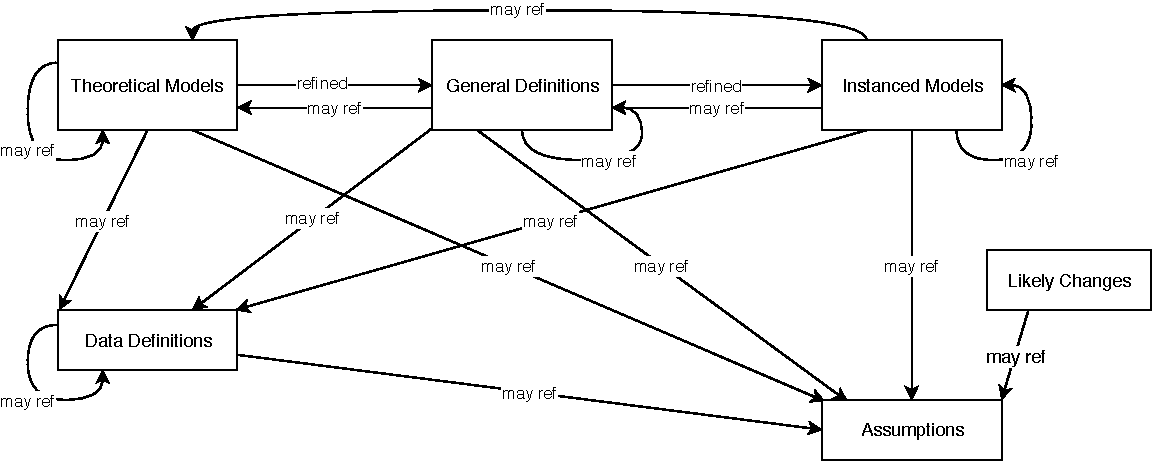
\includegraphics[scale=0.9]{RelationsBetweenTM_GD_IM_DD_A.pdf}
\end{figure}

}

\plt{
The instance models that govern \progname{f} are presented in
Subsection~\ref{sec_instance}.  The information to understand the meaning of the
instance models and their derivation is also presented, so that the instance
models can be verified.
}

\subsubsection{Assumptions} \label{sec_assumpt}

\plt{The assumptions are a refinement of the scope.  The scope is general, where
  the assumptions are specific.  All assumptions should be listed, even those
  that domain experts know so well that they are rarely (if ever) written down.}
\plt{The document should not take for granted that the reader knows which
  assumptions have been made. In the case of unusual assumptions, it is
  recommended that the documentation either include, or point to, an explanation
  and justification for the assumption.}

\plt{This section simplifies the original problem and helps in developing the
theoretical model by filling in the missing information for the physical
system. The numbers given in the square brackets refer to the theoretical model
[T], general definition [GD], data definition [DD], instance model [IM], or
likely change [LC], in which the respective assumption is used.}

Given a tolerance \tol, consider the sequence $\Setbg{c_n}$ and its power series
$\sum_{n=0}^{\infty} c_n (z-z_0)^n$
under the following assumptions:

\begin{itemize}

\plt{
\item[A\refstepcounter{assumpnum}\theassumpnum \label{A_meaningfulLabel}:]
  \plt{Short description of each assumption.  Each assumption
    should have a meaningful label.  Use cross-references to identify the
    appropriate traceability to T, GD, DD etc., using commands like dref, ddref
    etc.  Each assumption should be atomic - that is, there should not be an
    explicit (or implicit) ``and'' in the text of an assumption.}
}

\item[A\refstepcounter{assumpnum}\theassumpnum \label{as:n}:]
  We know an integer $N$ such that, for all $m \geq n \geq N$,
  $| \sum_{k=n}^{m} c_k | < \tol$.

\item[A\refstepcounter{assumpnum}\theassumpnum \label{as:approximate}:]
  The software \progname{f} will estimate the radius of convergence from a finite number of terms
  in the power series. It will not compute $R_c$ exactly. 

\item[A\refstepcounter{assumpnum}\theassumpnum \label{as:real}:]
  The sequence $\Setbg{c_n}$ is a subset of $\Rz$.

\item[A\refstepcounter{assumpnum}\theassumpnum \label{as:threeterm}:]
  The scope of three term analysis is to compute the radius of convergence of
  a real power series at a point $z_0 \in \Rz$ that has a primary singularity.

\item[A\refstepcounter{assumpnum}\theassumpnum \label{as:sixterm}:]
  The scope of six term analysis is to compute the radius of convergence of
  a real power series at a point $z_0 \in \Rz$ that has a complex conjugate pair of
  primary singularity.

\item[A\refstepcounter{assumpnum}\theassumpnum \label{as:topline}:]
  The scope of top line analysis is to compute the radius of convergence of
  a real power series at a point $z_0 \in \Rz$ that has a secondary singularity.

%\item[A\refstepcounter{assumpnum}\theassumpnum \label{as:linear-least-squares}:]
%  A Linear Least Squares fit to the input sequence approximates the Least Squares residual within \tol.

\end{itemize}

\subsubsection{Theoretical Models}\label{sec_theoretical}
\label{ssc:TM}

Applying the terminology and definitions from \SSCref{terminology-definitions}, this section records
theorems required to identify a convergent/divergent series.

Consider the sequence $\Setbg{c_n}$ and its power series $\sum_{n=0}^{\infty} c_n (z-z_0)^n$. The following
TM is used to show that the coefficients in the terms of a series tend to zero as the index of the term
tends to infinity.

\noindent
\begin{minipage}{\textwidth}
\renewcommand*{\arraystretch}{1.5}
\begin{tabular}{| p{\colAwidth} | p{\colBwidth}|}
  \hline
  \rowcolor[gray]{0.9}
  Number& T\refstepcounter{theorynum}\thetheorynum \label{TM-series-cauchy-condition}\\
  \hline
  Label&\bf Cauchy convergence condition\\
  \hline
  Theorem& A series $\sum_{n=0}^{\infty} c_n$ converges if an only if, for every $\epsilon > 0$,
  there is an integer $N$ such that $| \sum_{k=n}^{m} c_k | < \epsilon$ whenever $m \geq n \geq N$.\\ 
  \hline
  Description & Tools to identify when a series converges.\\
  \hline
  Source & Theorem 3.22 \cite[p.~59]{rudin1976}\\
  \hline
  Ref.\ By & \iref{IM-rc}\\
  \hline
\end{tabular}
\end{minipage}\\

~\newline

\noindent
\begin{minipage}{\textwidth}
\renewcommand*{\arraystretch}{1.5}
\begin{tabular}{| p{\colAwidth} | p{\colBwidth}|}
  \hline
  \rowcolor[gray]{0.9}
  Number& T\refstepcounter{theorynum}\thetheorynum \label{TM-convergence-of-sequence}\\
  \hline
  Label&\bf Convergence of sequence\\
  \hline
  Theorem& If series $\sum_{n=0}^{\infty} c_n$ converges, then $\lim_{n \rightarrow \infty} c_n = 0$.\\
  \hline
  Description & If a series converges, then its terms converge to zero.\\
  \hline
  Source & Theorem 3.28 \cite[p.~60]{rudin1976}\\
  \hline
  Ref.\ By & \iref{IM-rc}\\
  \hline
\end{tabular}
\end{minipage}\\

~\newline

\noindent
\begin{minipage}{\textwidth}
\renewcommand*{\arraystretch}{1.5}
\begin{tabular}{| p{\colAwidth} | p{\colBwidth}|}
  \hline
  \rowcolor[gray]{0.9}
  Number& T\refstepcounter{theorynum}\thetheorynum \label{TM-root-test}\\
  \hline
  Label&\bf Root test\\
  \hline
  Theorem&
  \begin{minipage}[t]{0.8\textwidth}  
    Given a series $\sum_{n=0}^{\infty} c_n$. Set $\alpha \defeq \nlimsup{n} \proot{n}{|c_n|}$.
  Then
  \begin{itemize}
    \item[(a)] if $\alpha < 1$, then $\sum_{n=0}^{\infty} c_n$ converges;
    \item[(b)] if $\alpha > 1$, then $\sum_{n=0}^{\infty} c_n$ diverges;
    \item[(c)] if $\alpha = 1$, then this test gives no information.
  \end{itemize}
  \end{minipage}\\
  \hline
  Description & Tools to identify when a series converges/diverges.\\
  \hline
  Source & Theorem 3.33 \cite[p.~65]{rudin1976}\\
  \hline
  Ref.\ By & \dref{GD-rc}\\
  \hline
\end{tabular}
\end{minipage}\\

~\newline

\noindent
\begin{minipage}{\textwidth}
\renewcommand*{\arraystretch}{1.5}
\begin{tabular}{| p{\colAwidth} | p{\colBwidth}|}
  \hline
  \rowcolor[gray]{0.9}
  Number& T\refstepcounter{theorynum}\thetheorynum \label{TM-ratio-test}\\
  \hline
  Label&\bf Ratio test\\
  \hline
  Theorem&
  \begin{minipage}[t]{0.8\textwidth} 
  The series $\sum_{n=0}^{\infty} c_n$
  \begin{itemize}
    \item[(a)] converges if $\nlimsup{n} \lvert \tfrac{c_{n+1}}{c_n} \rvert < 1$,
    \item[(b)] diverges if $\lvert \tfrac{c_{n+1}}{c_n} \rvert \geq 1$ for $n \geq N$, where $N$ is some fixed integer.
  \end{itemize}
  \end{minipage}\\
  \hline
  Description & Tools to identify when a series converges/diverges.\\
  \hline
  Source & Theorem 3.34 \cite[p.~66]{rudin1976}\\
  \hline
  Ref.\ By & \iref{IM-rc}\\
  \hline
\end{tabular}
\end{minipage}\\

~\newline
The ratio test is often easier to apply than the root test. However, the root test resolves more application
than the ratio test. Both the ratio test and the root test deduce divergence from the statement in
Theoretical Model \ref{TM-convergence-of-sequence}, if a series converges, then its terms converge to zero.
~\newline

\noindent
\begin{minipage}{\textwidth}
\renewcommand*{\arraystretch}{1.5}
\begin{tabular}{| p{\colAwidth} | p{\colBwidth}|}
  \hline
  \rowcolor[gray]{0.9}
  Number& T\refstepcounter{theorynum}\thetheorynum \label{TM-comparing-ratio-and-root}\\
  \hline
  Label&\bf Comparing the Ratio test and the Root test\\
  \hline
  Theorem& 
  \begin{minipage}[t]{0.8\textwidth} 
  For any sequence $\Setbg{c_n}$ of positive (real) numbers,
  \begin{itemize}
    \item[(a)] $\nliminf{n} \tfrac{c_{n+1}}{c_n} \leq \nliminf{n}\proot{n}{c_n}$,
    \item[(b)] $\nlimsup{n}\proot{n}{c_n} \leq \nlimsup{n} \tfrac{c_{n+1}}{c_n}$
  \end{itemize}
  \end{minipage}\\
  \hline
  Description & If the ratio test converges,
  then the root test converges and if the root test is inconclusive, then the ratio test is inconclusive.
  Whenever the limit exists and it is unique, then there is equality in (a) and (b) and
  $\lim_{n \rightarrow \infty} \tfrac{c_{n+1}}{c_n} = \lim_{n \rightarrow \infty} \proot{n}{c_n}$.
  \\
  \hline
  Source & Theorem 3.37 \cite[p.~68]{rudin1976}\\
  \hline
  Ref.\ By & \iref{IM-rc}\\
  \hline
\end{tabular}
\end{minipage}\\

~\newline

\plt{Theoretical models are sets of abstract mathematical equations or axioms
  for solving the problem described in Section ``Physical System Description''
  (Section~\ref{sec_phySystDescrip}). Examples of theoretical models are
  physical laws, constitutive equations, relevant conversion factors, etc.}

\plt{
This section focuses on the general equations and laws that \progname{f} is based
on.  \plt{Modify the examples below for your problem, and add additional models
  as appropriate.}
}

\plt{
~\newline

\noindent
\begin{minipage}{\textwidth}
\renewcommand*{\arraystretch}{1.5}
\begin{tabular}{| p{\colAwidth} | p{\colBwidth}|}
  \hline
  \rowcolor[gray]{0.9}
  Number& T\refstepcounter{theorynum}\thetheorynum \label{T_COE}\\
  \hline
  Label&\bf Conservation of thermal energy\\
  \hline
  Equation&  $-{\bf \nabla \cdot q} + g$ = $\rho C \frac{\partial T}{\partial t}$\\
  \hline
  Description & 
                The above equation gives the conservation of energy for transient heat transfer in a material
                of specific heat capacity $C$ (\si{\joule\per\kilogram\per\celsius}) and density $\rho$ 
                (\si{\kilogram\per\cubic\metre}), where $\bf q$ is the thermal flux vector (\si{\watt\per\square\metre}),
                $g$ is the volumetric heat generation
                (\si{\watt\per\cubic\metre}), $T$ is the temperature
                (\si{\celsius}),  $t$ is time (\si{\second}), and $\nabla$ is
                the gradient operator.  For this equation to apply, other forms
                of energy, such as mechanical energy, are assumed to be negligible in the
                system (\aref{A_OnlyThermalEnergy}).  In general, the material properties ($\rho$ and $C$) depend on temperature.\\
  \hline
  Source &
           \url{http://www.efunda.com/formulae/heat_transfer/conduction/overview_cond.cfm}\\
  % The above web link should be replaced with a proper citation to a publication
  \hline
  Ref.\ By & \dref{ROCT}\\
  \hline
\end{tabular}
\end{minipage}\\

~\newline
}

\subsubsection{General Definitions}\label{sec_gendef}

The proofs of the theorem in this section apply the terminology and definitions
from \SSCref{terminology-definitions} as well as the Theoretical models from \SSCref{TM}.

The radius of the circle of convergence is defined in the next General Definition, a theorem
that enables us to justify and construct the IM so that \progname{f} will estimate $R_c$.
~\newline

\noindent
\begin{minipage}{\textwidth}
\renewcommand*{\arraystretch}{1.5}
\begin{tabular}{| p{\colAwidth} | p{\colBwidth}|}
  \hline
  \rowcolor[gray]{0.9}
  Number& GD\refstepcounter{defnum}\thedefnum \label{GD-rc}\\
  \hline
  Label&\bf Define the radius of the circle of convergence\\
  \hline
  Theorem& Given any sequence $\Setbg{c_n}$, construct the power series
  $\sum_{n=0}^{\infty} c_n (z-z_0)^n$. Set $\alpha \defeq \nlimsup{n} \proot{n}{|c_n|}$ and $R_c \defeq 1/\alpha$.
  Then $\sum_{n=0}^{\infty} c_n (z-z_0)^n$ converges whenever $|z - z_0| < R_c$.\\
  \hline
  Description & This General Definition defines $R_c$, the radius of convergence of the power series.
  By our convention stated \SSCref{terminology-definitions}, $\alpha = 0$ implies $R_c = +\infty$ and
  $\alpha = +\infty$ implies $R_c = 0$.\\
  \hline
  Source & Theorem 3.39 \cite[p.~69]{rudin1976}\\
  \hline
  Ref.\ By & \iref{IM-rc}\\
  \hline
\end{tabular}
\end{minipage}\\

~\newline
We need to relate the root test to the ratio test to obtain our IM. It is instructive to
understand the role of the root test in the proof of \dref{GD-rc}.

\subsubsection*{Inside \dref{GD-rc}}

Given any sequence $\Setbg{c_n}$, construct the power series
$\sum_{n=0}^{\infty} c_n (z-z_0)^n$. Set $a_n = c_n (z - z_0)^n$, and apply the root test \tref{TM-root-test}
to the series $\sum_{n=0}^{\infty} a_n$.
\EQ
{
  \label{eq:rc-definition}
  \nlimsup{n} \proot{n}{|a_n|} = |z-z_0| \nlimsup{n} \proot{n}{|c_n|} \defeq \tfrac{|z-z_0|}{R_c}.
}
Obtain from the root test that
\begin{itemize}
  \item[(a)] if $|z-z_0| < R_c$, then the power series converges;
  \item[(b)] if $|z-z_0| > R_c$, then the power series diverges;
  \item[(c)] if $|z-z_0| = R_c$, then this test gives no information.
\end{itemize}

The next section presents a Data Definition on order of singularity.

\plt{General Definitions (GDs) are a refinement of one or more TMs, and/or of
  other GDs.  The GDs are less abstract than the TMs.  Generally the reduction
  in abstraction is possible through invoking (using/referencing) Assumptions.
  For instance, the TM could be Newton's Law of Cooling stated abstracting.  The
  GD could take the general law and apply it to get a 1D equation.}

\plt{
This section collects the laws and equations that will be used in building the
instance models.
}

\plt{Some projects may not have any content for this section, but the section
  heading should be kept.}  \plt{Modify the examples below for your problem, and
  add additional definitions as appropriate.}

\plt{
~\newline

\noindent
\begin{minipage}{\textwidth}
\renewcommand*{\arraystretch}{1.5}
\begin{tabular}{| p{\colAwidth} | p{\colBwidth}|}
\hline
\rowcolor[gray]{0.9}
Number& GD\refstepcounter{defnum}\thedefnum \label{NL}\\
\hline
Label &\bf Newton's law of cooling \\
\hline
% Units&$MLt^{-3}T^0$\\
% \hline
SI Units&\si{\watt\per\square\metre}\\
\hline
Equation&$ q(t) = h \Delta T(t)$  \\
\hline
Description &
Newton's law of cooling describes convective cooling from a surface.  The law is
stated as: the rate of heat loss from a body is proportional to the difference
in temperatures between the body and its surroundings.
\\
& $q(t)$ is the thermal flux (\si{\watt\per\square\metre}).\\
& $h$ is the heat transfer coefficient, assumed independent of $T$ (\aref{A_hcoeff})
	(\si{\watt\per\square\metre\per\celsius}).\\
&$\Delta T(t)$= $T(t) - T_{\text{env}}(t)$ is the time-dependent thermal gradient
between the environment and the object (\si{\celsius}).
\\
\hline
  Source & Citation here \\
  \hline
  Ref.\ By & \ddref{FluxCoil}, \ddref{FluxPCM}\\
  \hline
\end{tabular}
\end{minipage}\\
}

\plt{
\subsubsection*{Detailed derivation of simplified rate of change of temperature}
}

\plt{This may be necessary when the necessary information does not fit in the
  description field.}
\plt{Derivations are important for justifying a given GD.  You want it to be
  clear where the equation came from.}

\subsubsection{Data Definitions}\label{sec_datadef}

We quoted from \cite{chang1982} in \SCref{scope}, the scope section, that,
in general, the coefficients of a power series follow no patterns, so few theorems about truncated
series can be proved. However, series which are real-valued on the real axis can have poles,
logarithmic branch points, and essential singularities only on the real axis or in conjugate pairs.
The sequence $\Setbg{c_n}$ is a subset of $\Rz$ under \ASref{real}.
~\newline

\noindent
\begin{minipage}{\textwidth}
\renewcommand*{\arraystretch}{1.5}
\begin{tabular}{| p{\colAwidth} | p{\colBwidth}|}
\hline
\rowcolor[gray]{0.9}
Number& DD\refstepcounter{datadefnum}\thedatadefnum \label{DD-order-of-singularity}\\
\hline
Label& \bf Order of singularity\\
\hline
Symbol &$\mu$\\
\hline
  Conditions &
  Assume \ASref{real}.
Further assume the real coefficients $\Setbg{c_n} \subset \Rz$ of the power series
$\sum_{n=0}^{\infty} c_n (z-z_0)^n$ are obtained as a TS solution of an \ode and
consider finding the order $\mu$ of the singularity from the graph
of $\log_{10} | c_n |$ versus $n$.\\
\hline
  Observations &
  \begin{minipage}[t]{0.8\textwidth} 
The order $\mu$ is increased or decreased by term-by-term differentiation or
integration, respectively. The upper envelope of the graph of
$\log_{10} | c_n |$ versus $n$ will follow the following patterns:
\begin{itemize}
  \item If the order of the primary singularity, the closest singularity to $z_0$, is $\mu = 1$,
    then the slope is $\log_{10} |z - z_0|/R_c$.
    
  \item If the order of the primary singularity $\mu \neq 1$, then the slope converges to
    $\log_{10} |z - z_0|/R_c$ at a rate proportional to $1/n$.

  \item If the order of the primary singularity $\mu \neq 1$, then the upper envelope is not linear.
    For orders $\mu > 1$, the graph opens downward. The concavity approaches zero as
    $1/n^2$ as $n \rightarrow \infty$. For orders $\mu < 1$, the graph is concave up which means
    the slope underestimates $\log_{10} |z - z_0|/R_c$, and $R_c$ is overestimated.
\end{itemize}
  \end{minipage}\\
  \hline
Description &\\
  \hline
  Sources& Chang and Corliss \cite{chang1982}\\
  \hline
  Ref.\ By & \iref{IM-order-of-singularity}\\
  \hline
\end{tabular}
\end{minipage}\\

The next section derives an IM to approximate $R_c$.

\plt{The Data Definitions are definitions of symbols and equations that are
  given for the problem.  They are not derived; they are simply used by other
  models.  For instance, if a problem depends on density, there may be a data
  definition for the equation defining density.  The DDs are given information
  that you can use in your other modules.}

\plt{All Data Definitions should be used (referenced) by at least one other
  model.}

\plt{
This section collects and defines all the data needed to build the instance
models. The dimension of each quantity is also given.  \plt{Modify the examples
  below for your problem, and add additional definitions as appropriate.}
}

\plt{
~\newline

\noindent
\begin{minipage}{\textwidth}
\renewcommand*{\arraystretch}{1.5}
\begin{tabular}{| p{\colAwidth} | p{\colBwidth}|}
\hline
\rowcolor[gray]{0.9}
Number& DD\refstepcounter{datadefnum}\thedatadefnum \label{FluxCoil}\\
\hline
Label& \bf Heat flux out of coil\\
\hline
Symbol &$q_C$\\
\hline
% Units& $Mt^{-3}$\\
% \hline
  SI Units & \si{\watt\per\square\metre}\\
  \hline
  Equation&$q_C(t) = h_C (T_C - T_W(t))$, over area $A_C$\\
  \hline
  Description & 
                $T_C$ is the temperature of the coil (\si{\celsius}).  $T_W$ is the temperature of the water (\si{\celsius}).  
                The heat flux out of the coil, $q_C$ (\si{\watt\per\square\metre}), is found by
                assuming that Newton's Law 
                of Cooling applies (\aref{A_Newt_coil}).  This law (\dref{NL}) is used on the surface of
                the coil, which has area $A_C$ (\si{\square\metre}) and heat 
                transfer coefficient $h_C$
                (\si{\watt\per\square\metre\per\celsius}).  This equation
                assumes that the temperature of the coil is constant over time (\aref{A_tcoil}) and that it does not vary along the length
                of the coil (\aref{A_tlcoil}).
  \\
  \hline
  Sources& Citation here \\
  \hline
  Ref.\ By & \iref{ewat}\\
  \hline
\end{tabular}
\end{minipage}\\
}

\subsubsection{Instance Models} \label{sec_instance}    
\label{ssc:instance-models}

This section transforms the problem defined in Section~\ref{Sec_pd} into 
one which can be translated into software. We will define finite sequences
and series to replace the infinite counterparts
identified in Sections~\ref{sec_theoretical} and~\ref{sec_gendef}.

A heuristically motivated top-line analysis produces a conservative estimate
for the radius of convergence $R_c$ from the slope of a linear upper envelope
of a graph of $\log_{10} | c_n |$ versus $n$ \cite{chang1982}. While no proof
is given in this paper, the following argument justifies their claim that
the slope approaches $\log_{10} |z - z_0|/R_c$ as $n \rightarrow \infty$.

\noindent
\begin{minipage}{\textwidth}
\renewcommand*{\arraystretch}{1.5}
\begin{tabular}{| p{\colAwidth} | p{\colBwidth}|}
  \hline
  \rowcolor[gray]{0.9}
  Number& IM\refstepcounter{instnum}\theinstnum \label{IM-rc}\\
  \hline
  Label& \bf Approximating the radius of convergence\\
  \hline
  Inputs & $N$ and approximation points \eqref{approximation-points} \\
  \hline
  Output& $R_c$ or confirmation of divergence.\\
  \hline
  Description& Approximate the radius of the circle of convergence, $R_c \approx 1/10^m$.\\
  \hline
  Sources& The full details are my own contribution. However the ideas are inspired by conversations
  with G. Corliss and N. Nedialkov.\\
  \hline
  Ref.\ By & \iref{IM-order-of-singularity}\\
  \hline
\end{tabular}
\end{minipage}\\

Given $\tol>0$ and any sequence $\Setbg{c_n}$, construct the power series
$\sum_{n=0}^{\infty} c_n (z-z_0)^n$.
Use \ASref{n} to obtain an integer $N$ such that,
for all $m \geq n \geq N$, $| \sum_{k=n}^{m} c_k | < \tol$.
It is no loss in generality to assume $N>30$, else replace $N$ with $30$.
\tref{TM-series-cauchy-condition} says that $\sum_{n=0}^{\infty} c_n$ converges.

We now invoke \ASref{approximate} and extract $15$ elements 
$\Setbg{c_{N-14}, c_{N-13}, \ldots, c_{N}}$ from the sequence.
With $k = i+N-14$, obtain the best linear fit $y(k) = m k + b$ in the $2$-norm to the points
\EQ
{
  \label{eq:approximation-points}
  \Setbg{(N-14, \log_{10} | c_{N-14} |), (N-13, \log_{10} |c_{N-13}|), \ldots, (N, \log_{10} |c_{N}|)},
}
that is, find $m$ and $b$ such that $\sum_{i=0}^{14} |\log_{10} |c_{i+N-14}| - y(i+N-14)|^2$ is minimized.
Because $\sum_{n=0}^{\infty} c_n$ converges, \tref{TM-convergence-of-sequence} says that
$c_n \rightarrow 0$ as $n \rightarrow \infty$. The model parameter $m$ will be negative.

Compute the ratio in the ratio test \tref{TM-ratio-test} with our model. Then 
\EQ
{
  \log_{10} \left| \tfrac{y(k+1)}{y(k)} \right| = \log_{10} | y(k+1) | - \log_{10} | y(k) | = m,
}
which is independent of $k$. By continuity of $\log_{10}$ and the best linear fit function $y$ as well as
$\log_{10} \left| \tfrac{y(k+1)}{y(k)} \right|$ approximates $\log_{10} \left| \tfrac{c_{k+1}}{c_k} \right|$,
we observe that $\log_{10} \left| \tfrac{y(k+1)}{y(k)} \right| \rightarrow m$ is approximately
$\log_{10} \left| \tfrac{c_{k+1}}{c_k} \right| \rightarrow m$. By \tref{TM-comparing-ratio-and-root},
the ratio test \tref{TM-ratio-test} converging implies the root test \tref{TM-root-test} converges, because
they converge to a single limit and the same limit. See description section of \tref{TM-comparing-ratio-and-root}.
It follows from \dref{GD-rc} that the power series converges whenever $m<0$ and diverges whenever $m>0$.
Moreover \dref{GD-rc} says $R_c = 1/10^m$. 

~\newline

\noindent
\begin{minipage}{\textwidth}
\renewcommand*{\arraystretch}{1.5}
\begin{tabular}{| p{\colAwidth} | p{\colBwidth}|}
  \hline
  \rowcolor[gray]{0.9}
  Number& IM\refstepcounter{instnum}\theinstnum \label{IM-order-of-singularity}\\
  \hline
  Label& \bf Compute $\mu$ the order of singularity and underestimate $R_c$\\
  \hline
  Inputs & Tolerance \tol, $N$, and approximation points \eqref{approximation-points} \\
  \hline
  Output& $R_c$ and $\mu$\\
  \hline
  Description&
Start with the series resulting from integration of the given series three times and
fit the coefficients with \iref{IM-rc}. If that graph is linear, meaning the minimizer has norm less
  than \tol, then the slope is accepted and the order of the singularity is 3. If the graph opens upward,
then the series is differentiated term-wise to reduce the second derivative of the graph, and
a new top-line fit is computed. This process is repeated, reducing $\mu$ by 1 each time,
  until the graph opens downward or until
seven term-wise differentiations have been tested. If seven term-wise differentiations have been
tested and each result in turn proves unsatisfactory, then the final estimate for $R_c$ is reduced
by 10 percent for a conservative estimate for $R_c$ and $\mu=-4$ is returned.\\
  \hline
  Sources& \cite{chang1982}\\
  \hline
  Ref.\ By & Final product.\\
  \hline
\end{tabular}
\end{minipage}\\


Let the conditions of Data Definition \ddref{DD-order-of-singularity} hold.
Then the real coefficients $\Setbg{c_n} \subset \Rz$ of the power series
$\sum_{n=0}^{\infty} c_n (z-z_0)^n$ are obtained as a TS solution of an \ode and
consider finding the order $\mu$ of the singularity from the graph
of $\log_{10} | c_n |$ versus $n$.

The order $\mu$ is increased or decreased by term-by-term differentiation or
integration, respectively. The upper envelope of the graph of
$\log_{10} | c_n |$ versus $n$ is concave up for orders $\mu < 1$ which means
the slope underestimates $\log_{10} |z - z_0|/R_c$, and $R_c$ is overestimated.

To estimate $R_c$ and the order $\mu$ form the graph of $\log_{10} | c_n |$ versus $n$,
shift the order of the series by repeated term-wise differentiation or integration. After
each shift, a linear upper envelope is fit with \iref{IM-rc}. The singularity may occur with any order.
However, it is unusual for a solution to a differential equation to have singularities whose 
order lies beyond $| \mu - 1 | \leq 3$ \cite{chang1982}.

~\newline

\plt{The motivation for this section is to reduce the problem defined in
  ``Physical System Description'' (Section~\ref{sec_phySystDescrip}) to one
  expressed in mathematical terms. The IMs are built by refining the TMs and/or
  GDs.  This section should remain abstract.  The SRS should specify the
  requirements without considering the implementation.}

\plt{
This section transforms the problem defined in Section~\ref{Sec_pd} into 
one which is expressed in mathematical terms. It uses concrete symbols defined 
in Section~\ref{sec_datadef} to replace the abstract symbols in the models 
identified in Sections~\ref{sec_theoretical} and~\ref{sec_gendef}.
}

\plt{
The goals \plt{reference your goals} are solved by \plt{reference your instance
  models}.  \plt{other details, with cross-references where appropriate.}
\plt{Modify the examples below for your problem, and add additional models as
  appropriate.}

~\newline

%Instance Model 1

\noindent
\begin{minipage}{\textwidth}
\renewcommand*{\arraystretch}{1.5}
\begin{tabular}{| p{\colAwidth} | p{\colBwidth}|}
  \hline
  \rowcolor[gray]{0.9}
  Number& IM\refstepcounter{instnum}\theinstnum \label{ewat}\\
  \hline
  Label& \bf Energy balance on water to find $T_W$\\
  \hline
  Input&$m_W$, $C_W$, $h_C$, $A_C$, $h_P$, $A_P$, $t_\text{final}$, $T_C$, 
  $T_\text{init}$, $T_P(t)$ from \iref{epcm}\\
  & The input is constrained so that $T_\text{init} \leq T_C$ (\aref{A_charge})\\
  \hline
  Output&$T_W(t)$, $0\leq t \leq t_\text{final}$, such that\\
  &$\frac{dT_W}{dt} = \frac{1}{\tau_W}[(T_C - T_W(t)) + {\eta}(T_P(t) - T_W(t))]$,\\
  &$T_W(0) = T_P(0) = T_\text{init}$ (\aref{A_InitTemp}) and $T_P(t)$ from \iref{epcm} \\
  \hline
  Description&$T_W$ is the water temperature (\si{\celsius}).\\
  &$T_P$ is the PCM temperature (\si{\celsius}).\\
  &$T_C$ is the coil temperature (\si{\celsius}).\\
  &$\tau_W = \frac{m_W C_W}{h_C A_C}$ is a constant (\si{\second}).\\
  &$\eta = \frac{h_P A_P}{h_C A_C}$ is a constant (dimensionless).\\
  & The above equation applies as long as the water is in liquid form,
  $0<T_W<100^o\text{C}$, where $0^o\text{C}$ and $100^o\text{C}$ are the melting
  and boiling points of water, respectively (\aref{A_OpRange}, \aref{A_Pressure}).
  \\
  \hline
  Sources& Citation here \\
  \hline
  Ref.\ By & \iref{epcm}\\
  \hline
\end{tabular}
\end{minipage}\\

%~\newline
}

\plt{
\subsubsection*{Derivation of ...}
}

\plt{The derivation shows how the IM is derived from the TMs/GDs.  In cases
  where the derivation cannot be described under the Description field, it will
  be necessary to include this subsection.}

\subsubsection{Input Data Constraints} \label{sec_DataConstraints}    

Given tolerance \tol, the number of terms of the sequence should be sufficient so that \ASref{n}
  holds. We must know an integer $N$ such that, for all $m \geq n \geq N$,
  $| \sum_{k=n}^{m} c_k | < \tol$. Moreover if this $N<30$, then set $N=30$ for a sufficient
  number of terms to do analysis.

As a second point, the terms in the sequence should not be near overflow/underflow. If this
is the case, then the algorithm will properly scaled the sequence.

\plt{

Table~\ref{TblInputVar} shows the data constraints on the input output
variables.  The column for physical constraints gives the physical limitations
on the range of values that can be taken by the variable.  The column for
software constraints restricts the range of inputs to reasonable values.  The
software constraints will be helpful in the design stage for picking suitable
algorithms.  The constraints are conservative, to give the user of the model the
flexibility to experiment with unusual situations.  The column of typical values
is intended to provide a feel for a common scenario.  The uncertainty column
provides an estimate of the confidence with which the physical quantities can be
measured.  This information would be part of the input if one were performing an
uncertainty quantification exercise.

The specification parameters in Table~\ref{TblInputVar} are listed in
Table~\ref{TblSpecParams}.

\begin{table}[!h]
  \caption{Input Variables} \label{TblInputVar}
  \renewcommand{\arraystretch}{1.2}
\noindent \begin{longtable*}{l l l l c} 
  \toprule
  \textbf{Var} & \textbf{Physical Constraints} & \textbf{Software Constraints} &
                             \textbf{Typical Value} & \textbf{Uncertainty}\\
  \midrule 
  $L$ & $L > 0$ & $L_{\text{min}} \leq L \leq L_{\text{max}}$ & 1.5 \si[per-mode=symbol] {\metre} & 10\%
  \\
  \bottomrule
\end{longtable*}
\end{table}

\noindent 
\begin{description}
\item[(*)] \plt{you might need to add some notes or clarifications}
\end{description}

\begin{table}[!h]
\caption{Specification Parameter Values} \label{TblSpecParams}
\renewcommand{\arraystretch}{1.2}
\noindent \begin{longtable*}{l l} 
  \toprule
  \textbf{Var} & \textbf{Value} \\
  \midrule 
  $L_\text{min}$ & 0.1 \si{\metre}\\
  \bottomrule
\end{longtable*}
\end{table}
}

\subsubsection{Properties of a Correct Solution} \label{sec_CorrectSolution}

\progname{f} does not have properties of a correct solution to state which are in
addition to the requirements.

\plt
{
\noindent
A correct solution must exhibit \plt{fill in the details}.  \plt{These
  properties are in addition to the stated requirements.  There is no need to
  repeat the requirements here.  These additional properties may not exist for
  every problem.  Examples include conservation laws (like conservation of
  energy or mass) and known constraints on outputs (which are usually summarized
  in tabular form.  A sample table is shown in Table~\ref{TblOutputVar}}

\begin{table}[!h]
\caption{Output Variables} \label{TblOutputVar}
\renewcommand{\arraystretch}{1.2}
\noindent \begin{longtable*}{l l} 
  \toprule
  \textbf{Var} & \textbf{Physical Constraints} \\
  \midrule 
  $T_W$ & $T_\text{init} \leq T_W \leq T_C$ (by~\aref{A_charge})
  \\
  \bottomrule
\end{longtable*}
\end{table}
}

\section{Requirements}\label{sc:requirements}

\plt{The requirements refine the goal statement.  They will make heavy use of
  references to the instance models.}

This section provides the functional requirements, the business tasks that the
software is expected to complete, and the nonfunctional requirements, the
qualities that the software is expected to exhibit.

\subsection{Functional Requirements}

\progname{f} is the implementation of \iref{IM-rc} in the complex case or
\iref{IM-order-of-singularity} in the real case for TS solutions of \ode.

\begin{itemize}
  \item[\rlabel{rIHardware}] Input acquisition via hardware.
  \item[\rlabel{rISoftware}] Input acquisition via software.
  \item[\rlabel{rIFormat}] Validate input format.
  \item[\rlabel{rIType}] Validate input type.

  \item[\rlabel{rAssumptions}] Inputs should satisfy the assumptions.
  \item[\rlabel{R_Inputs}] Inputs should be scaled to prevent overflow/underflow.
  
  \item[\rlabel{rOHardware}] Output via hardware.
  \item[\rlabel{rOSoftware}] Output via software.
  \item[\rlabel{rOFormat}] Output format.
  \item[\rlabel{rOType}] Output type.
  \item[\rlabel{rPARAM}] Parameter acquisition.
  \item[\rlabel{rPFormat}] Parameter format.
  \item[\rlabel{rPType}] Parameter type.
  \item[\rlabel{rPDistribution}] Parameter distribution.
  \item[\rlabel{rPConstraints}] Parameter constraints.
  \item[\rlabel{rPoleRealSolverAlgorithm}] Algorithm to find the distance to the nearest real pole.
  \item[\rlabel{rPoleComplexSolverAlgorithm}] Algorithm to find the distance to the nearest complex conjugate pair of poles.
  \item[\rlabel{rPoleComplicatedAlgorithm}] Algorithm to find the distance to the nearest pole in hard to resolve case.
  \item[\rlabel{rPoleRealSolver}] Find the distance to the nearest real pole.
  \item[\rlabel{rPoleComplexSolver}] Find the distance to the nearest complex conjugate pair of poles.
  \item[\rlabel{rPoleTopLine}] Find the distance to the nearest pole in hard to resolve case.
  \item[\rlabel{rROC}] Pole identification, distinguish a real pole from a complex conjugate pair of poles
    from a complicated situation.

  \item[\rlabel{R_Calculate}] \progname{f} should be developed in \cpp.

    \progname{f} should execute as fast as the \cite{chang1982} software \rdcon. The method developed in this
    project is expected to be independent of system constraints. However
    most TS methods are developed in \cpp or \fortran, the goto languages
    of scientific computing. Certainly a scripting language would not be
    sufficient for large systems.
  
  \item[\rlabel{R_VerifyRealOutput}] Compute the TS for the real valued
    function $1/(z-z_0)^{\mu}$ at $x_c$. The radius of convergence $R_c$
    and the order of singularity $\mu$ computed by \progname{f} should
    be $R_c = | x_c - z_0 |$ and order of singularity $\mu$.
   
 \item[\rlabel{R_VerifyComplexOutput}] Compute the TS for the real valued function
   $1/(1 + 25*(z-z_0)^2)^{\mu}$ at $x_c$. The radius of convergence $R_c$
    and the order of singularity $\mu$ computed by \progname{f} should
    be $R_c = \sqrt( x_c^2 + (1/5)^2 |$ and order of singularity $\mu$.
  
 \item[\rlabel{R_VerifyOutput}] Compute the TS for the real valued function
   $1/(1 + 25*(z-z_0)^2)^{\mu}$ at $x_0$. The radius of convergence $R_c$
    and the order of singularity $\mu$ computed by \progname{f} should
    require top line analysis and top line analysis should compute
    $R_c$. Top line analysis doesn't compute an order of singularity.

  \item[\rlabel{R_Output}] We must not overestimate $R_c$.
    
    If $R_c$ is overestimated, then the power-series is a divergence sum on the overestimation.
  
    In \ode solving by TS methods, underestimating $R_c$ is acceptable as an underestimation
    results in a slight increase in computational effort for solving an \ode \ivp.
\end{itemize}

\plt
{
\noindent \begin{itemize}

\item[R\refstepcounter{reqnum}\thereqnum \label{R_Inputs}:] \plt{Requirements
    for the inputs that are supplied by the user.  This information has to be
    explicit.}

\item[R\refstepcounter{reqnum}\thereqnum \label{R_OutputInputs}:] \plt{It isn't
    always required, but often echoing the inputs as part of the output is a
    good idea.}

\item[R\refstepcounter{reqnum}\thereqnum \label{R_Calculate}:] \plt{Calculation
    related requirements.}

\item[R\refstepcounter{reqnum}\thereqnum \label{R_VerifyOutput}:]
  \plt{Verification related requirements.}

\item[R\refstepcounter{reqnum}\thereqnum \label{R_Output}:] \plt{Output related
    requirements.}

\end{itemize}
}

\subsection{Nonfunctional Requirements}

\progname{f} does not have nonfunctional requirements to state at this time.

\plt{
\SCref{SecUserCharacteristics}
This section summarizes the knowledge/skills expected of the user.
  Measuring usability, which is often a required non-function requirement,
  requires knowledge of a typical user. 
}

\plt{List your nonfunctional requirements.  You may consider using a fit
  criterion to make them verifiable.}

\section{Likely Changes}    

\cite{chang1982} discussed two additional estimators for $R_c$ of TS solutions to \ode under
\ASref{real}. This should be implemented, if there is time.

\plt
{
\noindent \begin{itemize}

\item[LC\refstepcounter{lcnum}\thelcnum\label{LC_meaningfulLabel}:] \plt{Give
    the likely changes, with a reference to the related assumption (aref), as appropriate.}

\end{itemize}
}

\section{Unlikely Changes} 

\progname{f} does not have unlikely changes to state at this time.

\plt
{
\noindent \begin{itemize}

\item[LC\refstepcounter{lcnum}\thelcnum\label{UC_meaningfulLabel}:] \plt{Give
    the unlikely changes.  The design can assume that the changes listed will
    not occur.}

\end{itemize}
}

\section{Traceability Matrices and Graphs}

The purpose of the traceability matrices is to provide easy references on what
has to be additionally modified if a certain component is changed.  Every time a
component is changed, the items in the column of that component that are marked
with an ``X'' may have to be modified as well.  Table~\ref{Table:trace} shows the
dependencies of theoretical models, general definitions, data definitions, and
instance models with each other. Table~\ref{Table:R_trace} shows the
dependencies of instance models, requirements, and data constraints on each
other. Table~\ref{Table:A_trace} shows the dependencies of theoretical models,
general definitions, data definitions, instance models, and likely changes on
the assumptions.

\afterpage{
%\begin{landscape}
\begin{table}[h!]
\centering
\begin{tabular}{|c|c|c|c|}
\hline
	& \aref{as:n}& \aref{as:approximate}& \aref{as:real} \\
\hline
\tref{TM-series-cauchy-condition}        &  &  &  \\ \hline
\tref{TM-convergence-of-sequence}        &  &  &  \\ \hline
\tref{TM-root-test}                      &  &  &  \\ \hline
\tref{TM-ratio-test}                     &  &  &  \\ \hline
\tref{TM-comparing-ratio-and-root}       &  &  &  \\ \hline
\dref{GD-rc}                             &  &  &  \\ \hline
\ddref{DD-order-of-singularity}          &  &  &  \\ \hline
\iref{IM-rc}                             & x& x&  \\ \hline
\iref{IM-order-of-singularity}           & x& x& x\\
\hline
\end{tabular}
\caption{Traceability Matrix Showing the Connections\\ Between Assumptions and Other Items}
\label{Table:A_trace}
\end{table}
%\end{landscape}
}

\begin{table}[h!]
\centering
\begin{tabular}{|c|c|c|c|c|c|c|c|c|c|}
\hline        
	& \tref{TM-series-cauchy-condition} & \tref{TM-convergence-of-sequence} & \tref{TM-root-test} &
\tref{TM-ratio-test} & \tref{TM-comparing-ratio-and-root} & \dref{GD-rc} & \ddref{DD-order-of-singularity} &
\iref{IM-rc} & \iref{IM-order-of-singularity} \\
\hline
\tref{TM-series-cauchy-condition}  &x& & & & & & &x& \\ \hline
\tref{TM-convergence-of-sequence}  & &x& & & & & &x& \\ \hline
\tref{TM-root-test}                & & &x& & &x& & & \\ \hline
\tref{TM-ratio-test}               & & & &x& & & &x& \\ \hline
\tref{TM-comparing-ratio-and-root} & & & & &x& & &x& \\ \hline
\dref{GD-rc}                       & & & & & &x& &x& \\ \hline
\ddref{DD-order-of-singularity}    & & & & & & &x& &x\\ \hline
\iref{IM-rc}                       & & & & & & & &x&x\\ \hline
\iref{IM-order-of-singularity}     & & & & & & & & &x\\
\hline
\end{tabular}
\caption{Traceability Matrix Showing the Connections\\Between Items of Different Sections}
\label{Table:trace}
\end{table}

\begin{table}[h!]
\centering
\begin{tabular}{|c|c|c|c|c|c|c|}
\hline
	& \iref{IM-rc} & \iref{IM-order-of-singularity} & \rref{R_Inputs} & \rref{R_Calculate} & \rref{R_VerifyOutput} & \rref{R_Output} \\
\hline
\iref{IM-rc}                   &x&x&x&x&x&x \\ \hline
\iref{IM-order-of-singularity} & &x&x&x&x&x \\ \hline
\rref{R_Inputs}                & & &x& & &  \\ \hline
\rref{R_Calculate}             & & & &x& &  \\ \hline
\rref{R_VerifyOutput}          & & & & &x&  \\ \hline
\rref{R_Output}                & & & & & &x \\
\hline
\end{tabular}
\caption{Traceability Matrix Showing the Connections\\Between Requirements and Instance Models}
\label{Table:R_trace}
\end{table}

\plt
{
The purpose of the traceability matrices is to provide easy references on what
has to be additionally modified if a certain component is changed.  Every time a
component is changed, the items in the column of that component that are marked
with an ``X'' may have to be modified as well.  Table~\ref{Table:trace} shows the
dependencies of theoretical models, general definitions, data definitions, and
instance models with each other. Table~\ref{Table:R_trace} shows the
dependencies of instance models, requirements, and data constraints on each
other. Table~\ref{Table:A_trace} shows the dependencies of theoretical models,
general definitions, data definitions, instance models, and likely changes on
the assumptions.

\plt{You will have to modify these tables for your problem.}

\plt{The traceability matrix is challenging to maintain manually.  Please do
  your best.  In the future tools (like Drasil) will make this much easier.}

\afterpage{
\begin{landscape}
\begin{table}[h!]
\centering
\begin{tabular}{|c|c|c|c|c|c|c|c|c|c|c|c|c|c|c|c|c|c|c|c|}
\hline
	& \aref{A_OnlyThermalEnergy}& \aref{A_hcoeff}& \aref{A_mixed}& \aref{A_tpcm}& \aref{A_const_density}& \aref{A_const_C}& \aref{A_Newt_coil}& \aref{A_tcoil}& \aref{A_tlcoil}& \aref{A_Newt_pcm}& \aref{A_charge}& \aref{A_InitTemp}& \aref{A_OpRangePCM}& \aref{A_OpRange}& \aref{A_htank}& \aref{A_int_heat}& \aref{A_vpcm}& \aref{A_PCM_state}& \aref{A_Pressure} \\
\hline
\tref{T_COE}        & X& & & & & & & & & & & & & & & & & & \\ \hline
\tref{T_SHE}        & & & & & & & & & & & & & & & & & & & \\ \hline
\tref{T_LHE}        & & & & & & & & & & & & & & & & & & & \\ \hline
\dref{NL}           & & X& & & & & & & & & & & & & & & & & \\ \hline
\dref{ROCT}         & & & X& X& X& X& & & & & & & & & & & & & \\ \hline
\ddref{FluxCoil}    & & & & & & & X& X& X& & & & & & & & & & \\ \hline
\ddref{FluxPCM}     & & & X& X& & & & & & X& & & & & & & & & \\ \hline
\ddref{D_HOF}       & & & & & & & & & & & & & & & & & & & \\ \hline
\ddref{D_MF}        & & & & & & & & & & & & & & & & & & & \\ \hline
\iref{ewat}         & & & & & & & & & & & X& X& & X& X& X& & & X \\ \hline
\iref{epcm}         & & & & & & & & & & & & X& X& & & X& X& X& \\ \hline
\iref{I_HWAT}       & & & & & & & & & & & & & & X& & & & & X \\ \hline
\iref{I_HPCM}       & & & & & & & & & & & & & X& & & & & X & \\ \hline
\lcref{LC_tpcm}     & & & & X& & & & & & & & & & & & & & & \\ \hline
\lcref{LC_tcoil}    & & & & & & & & X& & & & & & & & & & & \\ \hline
\lcref{LC_tlcoil}   & & & & & & & & & X& & & & & & & & & & \\ \hline
\lcref{LC_charge}   & & & & & & & & & & & X& & & & & & & & \\ \hline
\lcref{LC_InitTemp} & & & & & & & & & & & & X& & & & & & & \\ \hline
\lcref{LC_htank}    & & & & & & & & & & & & & & & X& & & & \\
\hline
\end{tabular}
\caption{Traceability Matrix Showing the Connections Between Assumptions and Other Items}
\label{Table:A_trace}
\end{table}
\end{landscape}
}

\begin{table}[h!]
\centering
\begin{tabular}{|c|c|c|c|c|c|c|c|c|c|c|c|c|c|c|c|c|c|c|c|c|c|c|c|}
\hline        
	& \tref{T_COE}& \tref{T_SHE}& \tref{T_LHE}& \dref{NL}& \dref{ROCT} & \ddref{FluxCoil}& \ddref{FluxPCM} & \ddref{D_HOF}& \ddref{D_MF}& \iref{ewat}& \iref{epcm}& \iref{I_HWAT}& \iref{I_HPCM} \\
\hline
\tref{T_COE}     & & & & & & & & & & & & & \\ \hline
\tref{T_SHE}     & & & X& & & & & & & & & & \\ \hline
\tref{T_LHE}     & & & & & & & & & & & & & \\ \hline
\dref{NL}        & & & & & & & & & & & & & \\ \hline
\dref{ROCT}      & X& & & & & & & & & & & & \\ \hline
\ddref{FluxCoil} & & & & X& & & & & & & & & \\ \hline
\ddref{FluxPCM}  & & & & X& & & & & & & & & \\ \hline
\ddref{D_HOF}    & & & & & & & & & & & & & \\ \hline
\ddref{D_MF}     & & & & & & & & X& & & & & \\ \hline
\iref{ewat}      & & & & & X& X& X& & & & X& & \\ \hline
\iref{epcm}      & & & & & X& & X& & X& X& & & X \\ \hline
\iref{I_HWAT}    & & X& & & & & & & & & & & \\ \hline
\iref{I_HPCM}    & & X& X& & & & X& X& X& & X& & \\
\hline
\end{tabular}
\caption{Traceability Matrix Showing the Connections Between Items of Different Sections}
\label{Table:trace}
\end{table}

\begin{table}[h!]
\centering
\begin{tabular}{|c|c|c|c|c|c|c|c|}
\hline
	& \iref{ewat}& \iref{epcm}& \iref{I_HWAT}& \iref{I_HPCM}& \ref{sec_DataConstraints}& \rref{R_RawInputs}& \rref{R_MassInputs} \\
\hline
\iref{ewat}            & & X& & & & X& X \\ \hline
\iref{epcm}            & X& & & X& & X& X \\ \hline
\iref{I_HWAT}          & & & & & & X& X \\ \hline
\iref{I_HPCM}          & & X& & & & X& X \\ \hline
\rref{R_RawInputs}     & & & & & & & \\ \hline
\rref{R_MassInputs}    & & & & & & X& \\ \hline
\rref{R_CheckInputs}   & & & & & X& & \\ \hline
\rref{R_OutputInputs}  & X& X& & & & X& X \\ \hline
\rref{R_TempWater}     & X& & & & & & \\ \hline 
\rref{R_TempPCM}       & & X& & & & & \\ \hline
\rref{R_EnergyWater}   & & & X& & & & \\ \hline
\rref{R_EnergyPCM}     & & & & X& & & \\ \hline
\rref{R_VerifyOutput}  & & & X& X& & & \\ \hline
\rref{R_timeMeltBegin} & & X& & & & & \\ \hline
\rref{R_timeMeltEnd}   & & X& & & & & \\ 
\hline
\end{tabular}
\caption{Traceability Matrix Showing the Connections Between Requirements and Instance Models}
\label{Table:R_trace}
\end{table}

The purpose of the traceability graphs is also to provide easy references on
what has to be additionally modified if a certain component is changed.  The
arrows in the graphs represent dependencies. The component at the tail of an
arrow is depended on by the component at the head of that arrow. Therefore, if a
component is changed, the components that it points to should also be
changed. Figure~\ref{Fig_ATrace} shows the dependencies of theoretical models,
general definitions, data definitions, instance models, likely changes, and
assumptions on each other. Figure~\ref{Fig_RTrace} shows the dependencies of
instance models, requirements, and data constraints on each other.
}

\plt{
\begin{figure}[h!]
	\begin{center}
		%\rotatebox{-90}
		{
			\includegraphics[width=\textwidth]{ATrace.png}
		}
		\caption{\label{Fig_ATrace} Traceability Matrix Showing the Connections Between Items of Different Sections}
	\end{center}
\end{figure}


\begin{figure}[h!]
	\begin{center}
		%\rotatebox{-90}
		{
			\includegraphics[width=0.7\textwidth]{RTrace.png}
		}
		\caption{\label{Fig_RTrace} Traceability Matrix Showing the Connections Between Requirements, Instance Models, and Data Constraints}
	\end{center}
\end{figure}
}

\section{Values of Auxiliary Constants}

\progname{f} does not have symbolic parameters at this time.

\plt{Show the values of the symbolic parameters introduced in the report.}

\plt{The definition of the requirements will likely call for SYMBOLIC\_CONSTANTS.
Their values are defined in this section for easy maintenance.}

\newpage

\bibliographystyle {plainnat}
\bibliography {../../refs/References}

\plt
{
\newpage
}

\noindent \plt{The following is not part of the template, just some things to consider
  when filing in the template.}

\noindent \plt{Grammar, flow and \LaTeX advice:
\begin{itemize}
\item For Mac users \texttt{*.DS\_Store} should be in \texttt{.gitignore}
\item \LaTeX{} and formatting rules
\begin{itemize}
\item Variables are italic, everything else not, includes subscripts (link to
  document)
\begin{itemize}
\item \href{https://physics.nist.gov/cuu/pdf/typefaces.pdf}{Conventions}
\item Watch out for implied multiplication
\end{itemize}
\item Use BibTeX
\item Use cross-referencing
\end{itemize}
\item Grammar and writing rules
\begin{itemize}
\item Acronyms expanded on first usage (not just in table of acronyms)
\item ``In order to'' should be ``to''
\end{itemize}
\end{itemize}}

\noindent \plt{Advice on using the template:
\begin{itemize}
\item Difference between physical and software constraints
\item Properties of a correct solution means \emph{additional} properties, not
  a restating of the requirements (may be ``not applicable'' for your problem).
  If you have a table of output constraints, then these are properties of a
  correct solution.
\item Assumptions have to be invoked somewhere
\item ``Referenced by'' implies that there is an explicit reference
\item Think of traceability matrix, list of assumption invocations and list of
  reference by fields as automatically generatable
\item If you say the format of the output (plot, table etc), then your
  requirement could be more abstract
\end{itemize}
}

\end{document}
